\documentclass{article}

\usepackage{fancyhdr}
\usepackage{extramarks}
\usepackage{amsmath}
\usepackage{amsthm}
\usepackage{amsfonts}
\usepackage{tikz}
\usepackage[plain]{algorithm}
\usepackage{algpseudocode}
\usepackage{tabularx}
\usepackage{hyperref}
\usepackage{subcaption}

\graphicspath{ {./img/} }
\newcolumntype{L}{>{\raggedright\arraybackslash}X}

\usetikzlibrary{automata,positioning}

%
% Basic Document Settings
%

\topmargin=-0.45in
\evensidemargin=0in
\oddsidemargin=0in
\textwidth=6.5in
\textheight=9.0in
\headsep=0.25in

\linespread{1.1}


\pagestyle{fancy}
\lhead{\hmwkAuthorName}
\chead{\hmwkClass\: \hmwkTitle}
\rhead{\firstxmark}
\lfoot{\lastxmark}
\cfoot{\thepage}

\renewcommand\headrulewidth{0.4pt}
\renewcommand\footrulewidth{0.4pt}

\setlength\parindent{0pt}

%
% Create Problem Sections
%

\newcommand{\enterProblemHeader}[1]{
    \nobreak\extramarks{}{Part \arabic{#1} continued on next page\ldots}\nobreak{}
    \nobreak\extramarks{Part \arabic{#1} (continued)}{Problem \arabic{#1} continued on next page\ldots}\nobreak{}
}

\newcommand{\exitProblemHeader}[1]{
    \nobreak\extramarks{Part \arabic{#1} (continued)}{Problem \arabic{#1} continued on next page\ldots}\nobreak{}
    \stepcounter{#1}
    \nobreak\extramarks{Part \arabic{#1}}{}\nobreak{}
}

\setcounter{secnumdepth}{0}
\newcounter{partCounter}
\newcounter{homeworkProblemCounter}
\setcounter{homeworkProblemCounter}{1}
\nobreak\extramarks{Part \arabic{homeworkProblemCounter}}{}\nobreak{}

%
% Homework Problem Environment
%
% This environment takes an optional argument. When given, it will adjust the
% problem counter. This is useful for when the problems given for your
% assignment aren't sequential. See the last 3 problems of this template for an
% example.
%
\newenvironment{homeworkProblem}[1][-1]{
    \ifnum#1>0
        \setcounter{homeworkProblemCounter}{#1}
    \fi
    \section{Part \arabic{homeworkProblemCounter}}
    \setcounter{partCounter}{1}
    \enterProblemHeader{homeworkProblemCounter}
}{
    \exitProblemHeader{homeworkProblemCounter}
}

%
% Homework Details
%   - Title
%   - Due date
%   - Class
%   - Section/Time
%   - Instructor
%   - Author
%

\newcommand{\hmwkTitle}{TD\ \#1}
\newcommand{\hmwkDueDate}{February 25, 2019}
\newcommand{\hmwkClass}{Algorithms for speech and natural language processing}
\newcommand{\hmwkClassTime}{}
\newcommand{\hmwkClassInstructor}{}
\newcommand{\hmwkAuthorName}{\textbf{ACHER Clément}}

%
% Title Page
%

\title{
    \vspace{2in}
    \textmd{\textbf{\hmwkClass:\ \hmwkTitle}}\\
    \normalsize\vspace{0.1in}\small{Due\ on\ \hmwkDueDate}\\
    \vspace{3in}
}

\author{\hmwkAuthorName}
\date{}

\renewcommand{\part}[1]{\textbf{\large Part \Alph{partCounter}}\stepcounter{partCounter}\\}

%
% Various Helper Commands
%

% Useful for algorithms
\newcommand{\alg}[1]{\textsc{\bfseries \footnotesize #1}}

% For derivatives
\newcommand{\deriv}[1]{\frac{\mathrm{d}}{\mathrm{d}x} (#1)}

% For partial derivatives
\newcommand{\pderiv}[2]{\frac{\partial}{\partial #1} (#2)}

% Integral dx
\newcommand{\dx}{\mathrm{d}x}

% Alias for the Solution section header
\newcommand{\solution}{\textbf{\large Solution}}

% Probability commands: Expectation, Variance, Covariance, Bias
\newcommand{\E}{\mathrm{E}}
\newcommand{\Var}{\mathrm{Var}}
\newcommand{\Cov}{\mathrm{Cov}}
\newcommand{\Bias}{\mathrm{Bias}}

\begin{document}

\maketitle

\pagebreak

\begin{homeworkProblem}
  The goal of this part is to build a classifier that given a voice command with
  a fixed length can recognize the spoken command. To achieve the best results, quite a
  few tricks can be used at various levels.

 \subsection{Feature extraction and feature engineering}
 The first thing I have done is to remove the cap on the number of samples used.
 Note that for the validation and test sets, this is almost necessary : 
 the proposed implementation will only extract samples from the first couple classes.
 They then can't be used to validate a model.\\

 \textbf{Tuning the speech features}
 
 It is pretty rare in ASR to feed a classifier with the raw signals. Features
 like MFCCs and Mel Filter Banks are more suited for such tasks. They however
 both rely on the choice of a few hyperparameters. To tune this features, I have
 mostly rely on the resources from
 \href{jhttp://practicalcryptography.com/miscellaneous/machine-learning/guide-mel-frequency-cepstral-coefficients-mfccs/}{this
   website}\footnote{http://practicalcryptography.com/miscellaneous/machine-learning/guide-mel-frequency-cepstral-coefficients-mfccs/}
 and the default parameters from another \href{https://python-speech-features.readthedocs.io/en/latest/}{feature extracting library}\footnote{https://python-speech-features.readthedocs.io/en/latest/} that I had
 used before.
 Table \ref{table:accuracy} shows the huge impact the choice of these parameters
 has : it shows the accuracy obtained using the two models initially included
 (no model tuning done at this point).
 
 \begin{table}[H]
    \centering
    \begin{tabularx}{\linewidth}{|L|L|L|L|L|}
      \hline
      Accuracy on val. set & MFCC - Initial parameters & Tuned MFCC - no normalization & Tuned MFCC - w/ normalization & Mel Filter Banks - w/ normalization\\
      \hline
      Log. Reg. & 3.6 & 14.92 & \textbf{30.46} & 10.42\\
      MLP & 39.4 & 53.68 & \textbf{65.92} & 52.66\\
      \hline
    \end{tabularx}
    \caption{Accuracy on vanilla models using different features}
    \label{table:accuracy}
  \end{table}

  \textbf{Normalization}

  Another factor of improvement that can be done at the feature level is about
  normalization. The idea is to get all the 13 features of the MFCC (or Mel
  filter banks) within the same range. As it can be seen on the Figure
  \ref{fig:nonorm}, the MFCC features are heavily dominated by the first
  coefficient. The 3 datasets are then normalized using the mean and the
  standard deviations of each coefficients across the whole training set. Note
  that there are other possibilities to normalize the datasets. Normalized MFCCs
  can be seen on the Figure \ref{fig:norm}. Normalization
  has a positive impact on the accuracy of the classifiers as shown in table
  \ref{table:accuracy}. The MLP classifier also converges faster (21 iterations
  vs. 29).

\begin{figure}[htbp]
    \centering
    \begin{subfigure}[b]{0.45\textwidth}
        \centering 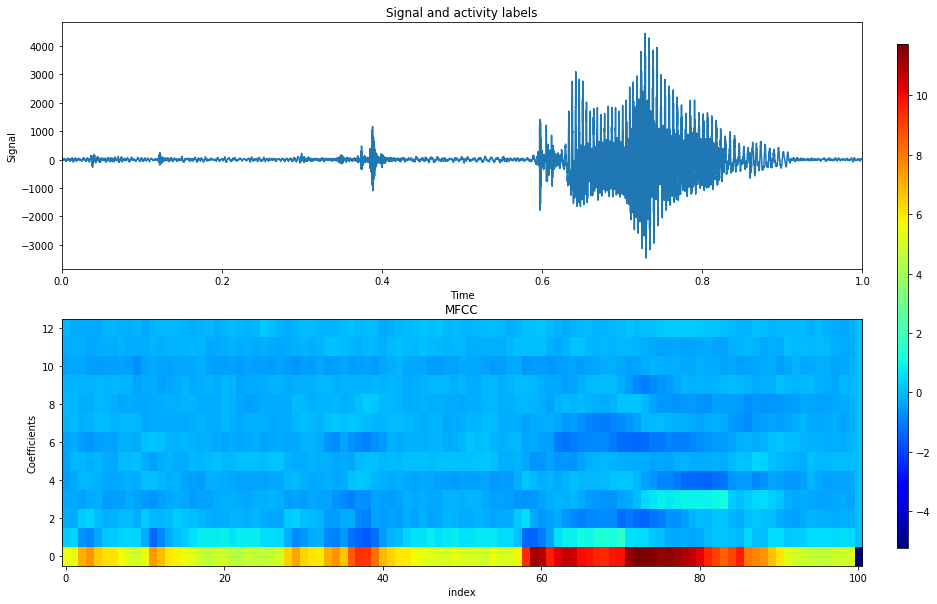
\includegraphics[width=\textwidth]{no_norm.png}
        \caption{No normalization}
        \label{fig:nonorm}
    \end{subfigure}
    ~ % ce symbole ajoute un espacement horisontal entre les premières deux images
    \begin{subfigure}[b]{0.45\textwidth}
        \centering 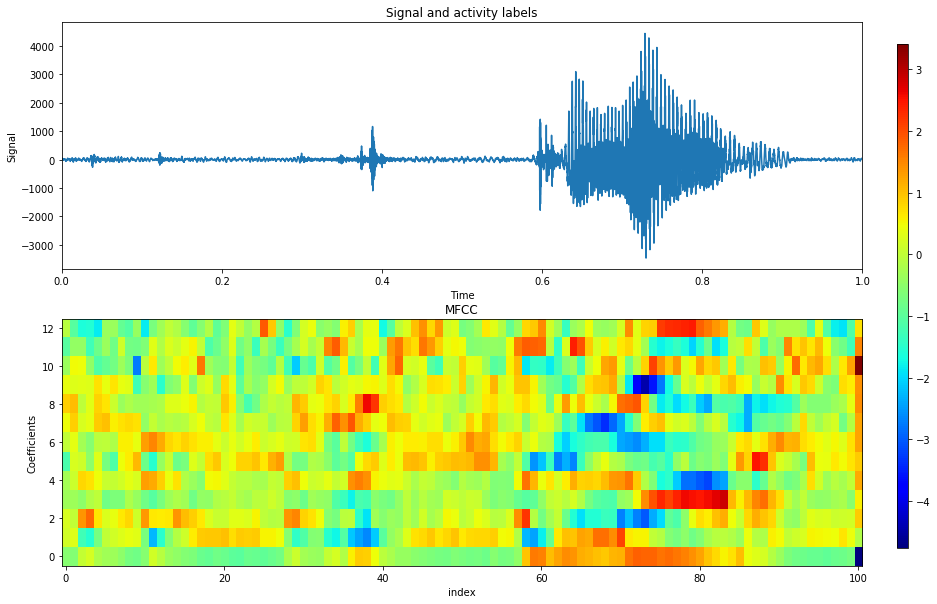
\includegraphics[width=\textwidth]{norm.png}
        \caption{With normalization}
        \label{fig:norm}
    \end{subfigure}
    \caption{Raw signal (top) and MFCC feature (bottom) with and without
      normalization.}\label{fig:normalization}
  \end{figure}

  As MFCC features were giving the best results, I have decided to only use these.\\

  \textbf{Data augmentation}

  The dataset also provides various sounds that can be used to perform data
  augmentation. However, the voice command audio signal and the noise should not
  simply added : many noise are way louder than the voice command. Simply
  summing these signals makes the command inaudible. To weight the ``quantity''
  of noise to add, I use the ratio of the RMS of the two signals.
  
\end{homeworkProblem}

\begin{homeworkProblem}
  \textbf{Question 2.1}

  The numerator is a sum of positive integers, so the WER can't be negative. It
  can be greater than 100, for instance if the reference is 'I like apple' and
  hypothesis ``She really loves dogs and cats'', the WER is 200.\\
  

  \textbf{Question 2.2}

  $\texttt{train\_labels.count(label) < nb\_ex\_per\_class}$ ensures that the dataset
  used for training is balanced and then that the prior probability of each word
  is equal.\\

  \textbf{Question 2.3}

  We have the following output:
  \begin{center}
    \texttt{True sentence:  go marvin one right stop}

    \texttt{Predicted sentence with greedy search: go marvin on five stop}
  \end{center}
  There are 2 substitutions out of the 5 words. The WER is then $\frac{2}{5} =
  0.4$.\\

  \textbf{Question 2.4}

  In the bigram model, we have:
  $$
    P ( W ) = \prod _ { k = 1 } ^ { T } P ( W _ { k } | W _ { k - 1 })
    $$\\

  \textbf{Question 2.5}

  The bigrams are stored in matrix $(P(w_k = j |w_{k-1} = i))_{i, j}$. To
  compute these probabilities, we go through all the sequences of the training
  set, and increment a the count of the encountered bigrams. The probabilities
  are then obtained by normalizing by the sum of the rows.\\
  On top of that, there are two extra tricks : Laplace smoothing (i.e. add 1 to
  every bigram counts) is used to avoid 0-counts. We also add an extra ``starting
  word'' at the beginning of each sequence so that there is a bigram for the
  first word of the sequence. We can notice this way that \texttt{go} is often
  the first word of the sequence.\\

  \textbf{Question 2.6}

  Increasing $N$ leads to a more accurate language model. However the number of
  entries in the transition matrix is $M^N$ where $M$ is the number of different
  possible words (31 here). The space complexity increases exponentially, and as
  the training dataset is rather small, it makes the matrix very sparse.\\

  \textbf{Question 2.7}

  We denote $L$ the length of a sequence ($L = 5$), $B$ the beam width and $M$
  the number of different words. The time complexity is then $\Theta({LBM(1 +
    \log(BM)))}$ if a sorting algorithm with complexity $\Theta(n\log(n))$ is used.\\
  

  \textbf{Question 2.8}

  
 
\end{homeworkProblem}

\end{document}